% Preprint — Sub-Family Dichotomy and Ladder Ceilings. Author: Derek Blair <derekjblair@gmail.com>
% Source data: ~/workspace/math-unsolved/ROUND245_DOSSIER.md (2026-10-09),
%              ~/workspace/math-unsolved/ROUND253_DOSSIER.md (2026-10-10),
%              ~/workspace/math-unsolved/ROUND256_DOSSIER.md (2026-10-10),
%              ~/workspace/math-unsolved/ROUND261_DOSSIER.md (2026-10-10),
%              ~/workspace/math-unsolved/ROUND262_DOSSIER.md (2026-10-10),
%              ~/workspace/math-unsolved/ROUND266_DOSSIER.md (2026-10-10),
%              ~/workspace/math-unsolved/ROUND274_DOSSIER.md (2026-10-10),
%              ~/workspace/math-unsolved/ROUND259_DOSSIER.md (2026-10-10),
%              ~/workspace/math-unsolved/ROUND263_DOSSIER.md (2026-10-10),
%              ~/workspace/math-unsolved/ROUND278_DOSSIER.md (2026-10-10),
%              ~/workspace/math-unsolved/ROUND310_DOSSIER.md (2026-10-11);
%              Lean modules ~/workspace/math-unsolved/lean/Mathproofs/ESSubfamilyExtended.lean
%              and ~/workspace/math-unsolved/lean/Mathproofs/MarchLadderCeiling.lean.
% All figures native TikZ/pgfplots; all tables booktabs.
\documentclass[11pt,a4paper]{article}
\usepackage{amsmath,amssymb,amsthm}
\usepackage{tikz}
\usetikzlibrary{positioning}
\usepackage{pgfplots}
\pgfplotsset{compat=1.18}
\usepackage{booktabs}
\usepackage{geometry}
\geometry{margin=2.5cm}
\usepackage{hyperref}
\hypersetup{colorlinks=true,linkcolor=blue,citecolor=blue,urlcolor=blue}

\newtheorem{theorem}{Theorem}
\newtheorem{proposition}{Proposition}
\newtheorem{lemma}{Lemma}
\newtheorem{corollary}{Corollary}
\theoremstyle{definition}
\newtheorem{assumption}{Assumption}

\title{Sub-Family Dichotomy and Ladder Ceilings:\\
  Generalized Erd\H{o}s--Straus Identities, Admission Pinning, and the
  March Ladder Bound}
\author{Derek Blair \\ \texttt{derekjblair@gmail.com}}
\date{October 2026}

\begin{document}
\maketitle

%======================================================================
\section{Abstract}
%======================================================================

The Erd\H{o}s--Straus conjecture asks for $4/n=1/x+1/y+1/z$ for every
$n\ge2$. This paper reports the generalized sub-family theorem of the
march-graph program (Round~245), its admission criterion (Round~253),
the $A_0$-constancy phenomenon (Round~261), the conditional
split/layered parent-set dichotomy (Rounds~256/265, repaired after a
reviewer refutation), and the two-sided ladder ceiling for hole-twin
march ladders (Rounds~259/263). The flagship result, machine-checked in
Lean, is the generalized sub-family identity
(Theorem~\ref{thm:general}): for every $s\ge1$ in the residue class
$s\equiv-m+4qeV_0\pmod{4qeA_0}$,
\begin{equation}
  \label{eq:general}
  \frac{4}{M't+s}=\frac{1}{x}+\frac{1}{nAC}+\frac{1}{BC}
  \qquad\forall t\ge0,
\end{equation}
with $M'=2042040\,q$, $S=510510\,q$, $x=XSTEP'\,t+x_0$,
$B=rt+w$, $C=pt+q_{\mathrm{par}}$, $n=M't+s$, an explicit infinite family
of Erd\H{o}s--Straus expansions [PROVED]. The admission criterion
(Theorem~\ref{thm:admit}, [PROVED*]: machine-checked, review-cleared,
full-library gate pending) characterizes, via prime valuations
$\alpha_p,\beta_p,\phi_p,\kappa_p$, exactly when a complementary divisor
$k\mid D_0$ is admitted; the $A_0$-constancy theorem
(Theorem~\ref{thm:a0}, [PROVED*]) shows admitted divisors determine a
shape-level constant $A_0$, hence a constant modulus $M(m)=4qeA_0(m)$.
The parent-set dichotomy is claimed only in its conditional,
same-modulus form (Theorem~\ref{thm:split}, [PROVED*]): the
unconditional version was refuted by an explicit counterexample
(Proposition~\ref{prop:uncond-false}: $q=29$, $A=10$, $r=510510$).
Finally the ladder ceiling (Theorem~\ref{thm:ladder6}, [PROVED]) bounds
hole-twin ladder length by the flanking isolation minus $185$, and the
catalog ceiling (Theorem~\ref{thm:catalog}, [PROVED]) gives $L\le9$ on
the $124$-base catalog, attained (ladder~49, [COMPUTED] datum).

%======================================================================
\section{Introduction}
%======================================================================

The Erd\H{o}s--Straus conjecture states that
\begin{equation}
  \label{eq:es}
  \frac{4}{n}=\frac{1}{x}+\frac{1}{y}+\frac{1}{z}
\end{equation}
is solvable in positive integers for every $n\ge2$~\cite{ES48,Mor69}.
The classical divisibility-collapse approach studies the denominator
through a ``cubic framework'' of parametrized divisor triples; this
program's march-graph track (Rounds~R59--R263) refines that framework
with the \emph{parent-set} mechanism of R209 and the \emph{hole-twin
ladder} machinery of R227/R231/R233. Within that track, the sub-family
program generalizes the R223 sub-family theorem (the $f=1$ case) to
arbitrary parameters: R245 proves a closed-form identity that produces
an entire residue-class of Erd\H{o}s--Straus expansions at once.

Concretely, fix $q\ge1$ and put
\begin{equation}
  \label{eq:params}
  S=510510\,q,\qquad M'=4S=2042040\,q.
\end{equation}
The integer setup (R245, \S\ref{sec:setup}) selects divisors
$A\mid S$ and $r\mid A\cdot S$, a minimal $e\ge1$ with $S\mid rqe$, and
$f=rqe/S\in\mathbb{Z}$; then $u=A\cdot S/r\in\mathbb{Z}$ and
$D_0=1+4u$. A complementary divisor $k\mid D_0$ with
$m=D_0/k\ge3$, $m\equiv3\pmod4$ drives the identity. The R245 identity
generalizes the R223 ($f=1$) family to the full two-parameter regime:
eight new-regime shapes with $f>1$ were verified with $1{,}239$ residue
hits and $0$ exceptions (supplied datum, R245 dossier).

Our contributions, with their honesty labels:
\begin{enumerate}
\item The generalized sub-family identity~\eqref{eq:general}, with the
  reviewer's relation chain, [PROVED] in Lean (Theorem~\ref{thm:general}).
\item The admission criterion in prime valuations, [PROVED*]
  (Theorem~\ref{thm:admit}), and its cluster corollary.
\item $A_0$-constancy for admitted complementary divisors, [PROVED*]
  (Theorem~\ref{thm:a0}), with the excess-prime pinning mechanism.
\item The split/layered parent-set dichotomy in conditional
  (same-modulus) form, [PROVED*] (Theorem~\ref{thm:split}), plus the
  honest record of the unconditional form's refutation
  (Proposition~\ref{prop:uncond-false}).
\item The two-sided ladder ceiling and the $L\le9$ catalog ceiling,
  both [PROVED] (Theorems~\ref{thm:ladder6} and~\ref{thm:catalog}).
\end{enumerate}
All [PROVED*] items are machine-checked with zero sorrys and have
survived rule-9 hostile review; their full-library build gate is
pending, so we present them with staged-verification language, never as
fully proved.

%======================================================================
\section{Methods}
%======================================================================

\subsection{Definitions and the identity setup}
\label{sec:setup}

We use the R245 setup verbatim (supplied datum, R245 dossier). Fix
$q\ge1$ and set $S$ and $M'$ as in~\eqref{eq:params}. Choose
$A\mid S$ and $r\mid A\cdot S$ (hence $r\mid S^2$, so the R72 TFAE
applies). Let $e\ge1$ be minimal with $S\mid rqe$ and put
$f=rqe/S\in\mathbb{Z}$; then $\gcd(e,f)=1$ and $r=Sf/(qe)$. Define
\begin{equation}
  \label{eq:uD0}
  u=\frac{A\cdot S}{r}\in\mathbb{Z},\qquad D_0=1+4u.
\end{equation}
For $m\ge3$ with $m\equiv3\pmod4$ and $m\mid D_0$, put $k=D_0/m$ (then
$k\equiv3\pmod4$ automatically, since $D_0\equiv1\pmod4$ and $3$ is
invertible mod~$4$) and
\begin{equation}
  \label{eq:A0}
  A_0=\frac{A}{\gcd(A,qek)}.
\end{equation}
If the congruence $(qek)V\equiv u\pmod A$ is solvable, let $V_0\pmod{A_0}$
be its unique solution. The branch-1 identity concerns every
$s\ge1$ with
\begin{equation}
  \label{eq:resclass}
  s\equiv-m+4qeV_0\pmod{4qeA_0},
\end{equation}
writing $V=(s+m)/(4qe)\ge1$, $x_0=qeV$, $w=fV$,
$p=(S/A)k$, $q_{\mathrm{par}}=(sk+1)/(4A)$, $c=(m+1)/4$, and
\begin{equation}
  \label{eq:branch1params}
  x=St+x_0,\qquad B=rt+w,\qquad C=pt+q_{\mathrm{par}},\qquad n=M't+s.
\end{equation}
The claimed identity is~\eqref{eq:general}, i.e.
$4/(M't+s)=1/x+1/(nAC)+1/(BC)$ for all $t\ge0$. It is proved in Lean
independently of the R72 TFAE, via the reviewer's relation chain
\begin{equation}
  \label{eq:chain}
  4x=n+m,\qquad B\cdot S=r\cdot x,\qquad 4AC=kn+1,\qquad mk=1+4u
\end{equation}
(supplied datum, R262 dossier).

For the admission criterion (R253) we track prime valuations
\begin{equation}
  \label{eq:valuations}
  \alpha_p=v_p(A),\qquad \beta_p=v_p(qe),\qquad
  \phi_p=v_p(f),\qquad \kappa_p=v_p(k).
\end{equation}
A prime $p$ is an \emph{excess prime} when $\phi_p<\alpha_p$. The
admission condition on the valuation quadruple is
\begin{align}
  \label{eq:AdmCond}
  \mathrm{AdmCond}(\alpha,\beta,\phi,\kappa)
  :=&\;(\beta\ge\alpha\to\phi\le\beta)\;\land\;
      \lnot(\beta<\alpha\land\phi>\alpha) \nonumber\\
  &\land\;(\beta<\alpha\to\phi=\alpha\to\kappa=0) \nonumber\\
  &\land\;(\beta<\alpha\to\beta<\phi\to\phi<\alpha\to\kappa\le\alpha-\phi),
\end{align}
with a fifth (``no condition'') case contributing nothing (supplied
datum, R253 dossier). In the cluster regime $f=A$ the criterion
collapses to the cluster corollary
$\gcd(D_0/m,A_{\mathrm{excess}})=1$ where
\begin{equation}
  \label{eq:Aexcess}
  A_{\mathrm{excess}}=\prod_{p:\,v_p(A)>v_p(qe)}p^{\,v_p(A)}.
\end{equation}

Parent-set machinery (R256, supplied datum; used as hypothesis, see
Assumption~\ref{asm:determ}): for $M_0=2042040$ (R209's modulus),
\begin{equation}
  \label{eq:parents}
  P(m)=\{s'\ \text{parent} : s'\equiv\mathrm{res}(m)\pmod{g(m)}\},
\end{equation}
$M(m)=4qeA_0(m)$,
$\mathrm{res}(m)=(-m+4qeV_0(m))\bmod M(m)$,
$g(m)=\gcd(M_0,M(m))$. Parent sets are \emph{split} when disjoint and
\emph{layered} when identical.

A \emph{hole-twin ladder} (R259) is a pair of rung sequences
$(X_t,Y_t)$, $t=0,\dots,L-1$ with $L=t_1-t_0+1$; side-$A$ rungs are
translates of a base $B_a$ whose march gap $g_a$ is flanked by neighbors
$g^a_{\mathrm{prev}}<g_a<g^a_{\mathrm{next}}$, side-$B$ analogously.
The \emph{isolation} is $g_{\mathrm{next}}-g_{\mathrm{prev}}$. Rung $s$
uses the window $[1-s,184-s]$; the rung-window union over $[t_0,t_1]$ is
$[1-t_1,184-t_0]$, which meets the shadow-gap set $G$ in exactly $\{g\}$
(formalized hypothesis of Theorem~\ref{thm:ladder6}). The catalog
universe (R259/R263): $62$ bases $\times$ raw/$\varphi$ $\times$ all
valid translates $=9{,}242$ translates; $124$ oriented bases;
$52$~marches (supplied datum).

\subsection{Formalization note}
\label{sec:formalization}

The machine-checked content lives in the repository
\texttt{derekblair/math-proofs}, Lean~4.34.1 with Mathlib pinned at
commit \texttt{d13f23b} (full pin
\texttt{d13f23b723b8a846827a245b89c10fc7d3f11612}).
Verification config: per-module and full-library \texttt{lake build} on
the bakkie fleet machine, exit~$0$, zero \texttt{sorry}s, zero
\texttt{admit}s, \texttt{\#print axioms} audits recorded per theorem.
The formalized results are:

\begin{table}[t]
  \centering
  \caption{Formalized theorems and their verification status. Module
    paths are repo-relative. [PROVED]: full build gate passed;
    [PROVED*]: machine-checked, review-cleared, full-library gate
    pending (staged verification).}
  \label{tab:formalization}
  \begin{tabular}{llp{5.2cm}}
    \toprule
    Lean theorem & status & verification \\
    \midrule
    \multicolumn{3}{l}{\texttt{Mathproofs/ESSubfamilyExtended.lean}} \\
    \ \ \texttt{generalized\_subfamily\_identity}
      & [PROVED]
      & local + bakkie exit~0 (R262); axioms
        \texttt{[propext, Classical.choice, Quot.sound]} \\
    \ \ \texttt{admission\_criterion}
      & [PROVED*]
      & bakkie exit~0 (R266); standard-only axioms \\
    \ \ \texttt{a0\_constancy} (+ \texttt{a0\_constancy\_formula},
        \texttt{u\_eq\_Aqe\_div\_f}, \texttt{excess\_prime\_dvd\_u},
        \texttt{pinning\_lemma}, \texttt{admission\_pinning},
        \texttt{M\_const})
      & [PROVED*]
      & bakkie exit~0 (R266); standard-only axioms
        (\texttt{u\_eq\_Aqe\_div\_f}: \texttt{[propext]} only) \\
    \ \ \texttt{split\_layered\_restated}
      & [PROVED*]
      & bakkie exit~0 (R266); standard-only axioms \\
    \ \ \texttt{split\_layered\_repaired}
      & [PROVED*]
      & bakkie exit~0 (R274); standard-only axioms \\
    \multicolumn{3}{l}{\texttt{Mathproofs/MarchLadderCeiling.lean}} \\
    \ \ \texttt{one\_sided\_ceiling}
      & [PROVED]
      & bakkie exit~0 (R278); axioms \texttt{[propext, Quot.sound]} \\
    \ \ \texttt{theorem6}
      & [PROVED]
      & bakkie exit~0; axioms \texttt{[propext, Quot.sound]} \\
    \ \ \texttt{catalog\_ceiling} (+ \texttt{\_nonbinding},
        \texttt{\_binding})
      & [PROVED]
      & bakkie exit~0 (R278); axioms \texttt{[propext, Quot.sound]} \\
    \bottomrule
  \end{tabular}
\end{table}

The R310 full-library gate (2026-10-11, 11:12~PDT) ran
\texttt{lake build} over the entire library on bakkie:
``Build completed successfully (17936 jobs)'' --- exit~$0$, $0$ errors,
$0$ \texttt{sorry}s in the log, with \texttt{MarchLadderCeiling} among
the modules built. Modules are md5-identical local~$\leftrightarrow$~bakkie
(\texttt{ESSubfamilyExtended.lean} \texttt{4df0b499d7c46ab24eeef8b6de6f480b}
after the R274 fold; \texttt{MarchLadderCeiling.lean}
\texttt{d9049f0dfb5b94a3e4f173b2407f6025}). Each module's header points
at this paper's slug
\texttt{papers/subfamily-ladder-ceiling-October-11-2026/}; this paper
points back at the modules and the exact theorem names of
Table~\ref{tab:formalization}. The census data cited as hypotheses in
Theorem~\ref{thm:catalog} (ledger values, attainment datum) are
[COMPUTED], not formalized. All [PROVED*] items were checked with zero
sorrys and survived rule-9 hostile review; their explicit full-library
label move is pending, so this paper presents them with
staged-verification language.

\subsection{Standing hypotheses}

\begin{assumption}[Parent-set determination]
  \label{asm:determ}
  The parent sets of~\eqref{eq:parents} are determined by the residue
  data: $P_i=\{s':s'\equiv\mathrm{res}_i\pmod{g}\}$ for the two shapes
  under comparison. This is cited from R256 as a hypothesis, not proved
  in the Lean modules; Theorems~\ref{thm:split} uses it explicitly.
  Its status is mixed (see Discussion): the R256 review accepted the
  arithmetic and CRT arguments but required the computed inputs, and the
  general ``$q\nmid m$'' premise is false as stated.
\end{assumption}

\begin{assumption}[Census ledger]
  \label{asm:ledger}
  The catalog figures used in Theorem~\ref{thm:catalog} are supplied
  [COMPUTED] datums (R263 dossier, [COMPUTED]$\times2$): distinct-base
  maximum $\min(\mathrm{iso}_A,\mathrm{iso}_B)=194$ (only
  R47\#15~$\times$~R47\#21, raw$\times$raw and $\varphi\times\varphi$);
  overlap $\le9$; attainment $L=9$ (ladder~49). The ladder hunt of R259
  ($202$ hole-twin pairs, $134$ single-gap, $60$ ladders) is likewise a
  supplied [COMPUTED] datum, not formalized.
\end{assumption}

%======================================================================
\section{Results}
%======================================================================

\begin{theorem}[Generalized sub-family identity; PROVED]
  \label{thm:general}
  Under the setup of~\S\ref{sec:setup} with explicit positivity
  $0<q$, $0<A$, $0<r$, $0<e$, $0<f$, $3\le m$, $m\equiv3\pmod4$, and
  $A\mid S$, $u\cdot r=A\cdot S$, $f\cdot S=r\cdot q\cdot e$,
  $m\cdot k=1+4u$, $qekV_0\equiv u\pmod A$,
  $s\equiv-m+4qeV_0\pmod{4qe(A/\gcd(A,qek))}$, $1\le s$: for every
  $t\ge0$,
  \begin{equation}
    \frac{4}{M't+s}
    =\frac{1}{S\,t+qe\,\frac{s+m}{4qe}}
     +\frac{1}{(M't+s)\,A\,\bigl(\frac{S}{A}k\,t+\frac{sk+1}{4A}\bigr)}
     +\frac{1}{\bigl(r\,t+f\,\frac{s+m}{4qe}\bigr)
               \bigl(\frac{S}{A}k\,t+\frac{sk+1}{4A}\bigr)}.
  \end{equation}
\end{theorem}

The denominators are positive for $t\ge0$ by the hypotheses; the proof
in Lean follows the relation chain~\eqref{eq:chain} supplied by the
reviewer and uses no divisibility-collapse machinery beyond it. The
positivity hypotheses $0<A$, $0<r$ were added at review: the literal
statement admits the counterexample $q=A=e=1$, $r=-510510$, $m=3$,
$s=1$ (supplied datum, R262 dossier), for which all written
divisibilities hold but the expansion's denominators collapse
($w=-1$, $q_{\mathrm{par}}=0$). The reviewed rule-9 verdict (Codex
gpt-6-astra/ultra) is SURVIVES under the positive-integer conventions.

\begin{table}[t]
  \centering
  \caption{The eight new-regime ($f>1$) shapes of R245: $1{,}239$ residue
    hits, $0$ exceptions, two independent code paths. Exact-identity
    batteries at $t\in\{0,1,2,3,7,10^5,10^9+7\}$ and
    $t\in\{0,2,5,11,10^6,10^9+9\}$ ($480$ evals), $0$ failures (supplied
    datum, R245 dossier).}
  \label{tab:r245shapes}
  \begin{tabular}{rrrcrrcl}
    \toprule
    $q$ & $A$ & $r$ & $e$ & $f$ & $u$ & $D_0$ & valid $m$ / observed \\
    \midrule
    29 & 10 & 5105100 & 1 & 10 & 29 & 117 & 3, 39 / 3 \\
    29 & 2  & 1021020 & 1 & 2  & 29 & 117 & 3, 39 / 3 \\
    29 & 5  & 2552550 & 1 & 5  & 29 & 117 & 3, 39 / 3 \\
    29 & 6  & 340340  & 3 & 2  & 261 & 1045 & 11, 55, 95 / 11 \\
    31 & 6  & 765765  & 2 & 3  & 124 & 497 & 7, 71 / 7 \\
    31 & 6  & 26180   & 39 & 2 & 3627 & 14509 & 11, 1319 / 11 \\
    31 & 2  & 60060   & 17 & 2 & 527 & 2109 & 3, 19, 111, 703 / 19 \\
    31 & 5  & 150150  & 17 & 5 & 527 & 2109 & 3, 19, 111, 703 / 111 \\
    \bottomrule
  \end{tabular}
\end{table}

\begin{theorem}[Admission criterion; PROVED*]
  \label{thm:admit}
  Let the setup of~\S\ref{sec:setup} hold with $f\mid A\cdot qe$.
  A complementary divisor $k\mid D_0$ is admitted iff for every prime
  $p$ the valuation quadruple~\eqref{eq:valuations} satisfies
  $\mathrm{AdmCond}$ of~\eqref{eq:AdmCond}:
  \begin{equation}
    \operatorname{Nat.gcd}\,A\,(qe\cdot k)\mid\frac{A\cdot qe}{f}
    \;\Longleftrightarrow\;
    \forall p\ \mathrm{prime},\;
    \mathrm{AdmCond}\bigl(A_p,(qe)_p,f_p,k_p\bigr).
  \end{equation}
  In the cluster regime $f=A$ this is equivalent to
  $\gcd(D_0/m,A_{\mathrm{excess}})=1$.
\end{theorem}

Theorem~\ref{thm:admit} is the R253 criterion, formalized in R266
(\texttt{admission\_criterion}, [PROVED*]): machine-checked on bakkie,
exit~$0$, zero sorrys, standard-only axioms; rule-9 review SURVIVES,
conditional on R245 supplying the integer setup (the Lean statement
carries it explicitly). The criterion matches brute-force solvability on
$154/154$ (shape, valid $m$) pairs, two code paths, $0$ disagreements
(supplied datum, R253 dossier). Example: the $\times29$ cluster
$qe=377=13\cdot29$, $u=377$, $D_0=3\cdot503$: $A=7$ admits $\{3,503\}$
(both observed); $A=6,3$ admit $\{3\}$ only (the excess prime $3$
divides $k=3$, killing $m=503$); $A=2$ admits $\{3,503\}$ but
$m=503$'s class has residue $-503+4\cdot377\cdot1=1005\equiv5\pmod8$ with
$\gcd(3016,24)=8$, so it is structurally parent-unreachable (all $196$
parents are $\equiv1\pmod8$) (supplied datum, R253 dossier).

\begin{theorem}[$A_0$-constancy; PROVED*]
  \label{thm:a0}
  In the setup of~\S\ref{sec:setup}: (i) $u=A\cdot qe/f$
  (\texttt{u\_eq\_Aqe\_div\_f}); (ii) at every excess prime $p$
  ($\phi_p<\alpha_p$), $p\mid u$, hence $p\nmid D_0=1+4u$, so any
  admitted $k$ has $\kappa_p=0$ (\texttt{excess\_prime\_dvd\_u},
  \texttt{pinning\_lemma}, \texttt{admission\_pinning}); (iii) every
  admitted complementary divisor gives the same shape-level constant
  $A/\gcd(A,qe\cdot k)=A/\gcd(A,qe)$
  (\texttt{a0\_constancy\_formula}); (iv) two admitted divisors
  $k_1,k_2$ determine the same $A_0$
  (\texttt{a0\_constancy}, \texttt{a0\_constancy\_admitted}); (v)
  $M(m)=4qeA_0(m)$ is shape-level constant (\texttt{M\_const}).
\end{theorem}

Theorem~\ref{thm:a0} is R261's A0-constancy suite, formalized in R266
([PROVED*]): bakkie exit~$0$, zero sorrys, standard-only axioms
(\texttt{u\_eq\_Aqe\_div\_f} uses \texttt{[propext]} alone); rule-9
review SURVIVES (``The A$_0$-constancy theorem survives''). Evidence
(supplied datum, R261 dossier): exhaustive census of $781{,}250$ shapes
($q\in\{29,31\}$, $A\mid510510q$, $r\mid A\cdot510510q$), $294{,}996$
multi-$m$; $A_0$ constant on every admitted set, $0$ counterexamples.
The pinning mechanism is sharp: on $410{,}008$ shapes with case-(d)/(e)
excess primes, $v_p(D_0)=0$ in $100\%$ (fingerprint, supplied datum).

\begin{theorem}[Conditional split/layered dichotomy; PROVED*]
  \label{thm:split}
  Assume Assumption~\ref{asm:determ}. Then
  $(P_1=P_2\iff\mathrm{res}_1\equiv\mathrm{res}_2\pmod g)$ and
  $(\mathrm{Disjoint}\,P_1\,P_2\iff\mathrm{res}_1\not\equiv
  \mathrm{res}_2\pmod g)$ hold unconditionally in the forward
  ($\Rightarrow$ replaced by the implication) directions, and hold in
  both directions under $(P_1\cup P_2)\neq\varnothing$
  (\texttt{split\_layered\_restated}, \texttt{split\_layered\_repaired}).
\end{theorem}

Precisely, \texttt{split\_layered\_repaired} (R265, folded R274,
[PROVED*]: bakkie exit~$0$, zero sorrys, standard-only axioms; Q-10
rule-9 review ``conditional SURVIVES'', $9/9$ checks) states the three
clauses: $\mathrm{res}_1\not\equiv\mathrm{res}_2\to\mathrm{Disjoint}$,
$\mathrm{res}_1\equiv\mathrm{res}_2\to P_1=P_2$, and both $\iff$s under
$(P_1\cup P_2).\mathrm{Nonempty}$. The determination premise itself is
\emph{not} proved (Assumption~\ref{asm:determ}); only the
residue-implication layer is machine-checked.

\begin{proposition}[Unconditional dichotomy refuted; COMPUTED]
  \label{prop:uncond-false}
  The unconditional split/layered $\iff$ corollary is false as stated.
  For $q=29$, $A=10$, $r=510510$ there are admitted values whose parent
  sets are empty: such sets are both identical and disjoint, breaking
  both $\iff$ directions (supplied datum, R261/R262 dossiers). Sharper
  (R265): for $A=10$ the four admitted $m$'s $\{3,27,43,387\}$ all have
  $P(m)=\varnothing$, giving $6/6$ converse failures (supplied datum).
\end{proposition}

This is R261's refuted corollary \texttt{split\_layered\_dichotomy\_
unconditional}: the rule-9 reviewer (verbatim) wrote ``The A$_0$-constancy
theorem survives. The appended corollary does not: both `$\iff$'
statements are false as written.'' Only the conditional,
same-modulus forms of Theorem~\ref{thm:split} are claimed. Separately,
the R256 review was MIXED on a different ground: the general premise
``$q\nmid m$'' is false (explicit admitted counterexample $q=29$,
$A=1$, $r=227766$, $m=87$ with $29\mid87$; supplied datum), and the
R209-base-unreachability repair is absent.

Multi-$m$ census (supplied datum, R256 dossier): $118/118$ admitted
pairs have predicted parent sets equal to observed, $0$ mismatches;
$302/302$ new-regime admitted pairs split; $6/6$ R223 pairs layered.
Examples: $29$ $(7,274890)$: $m$'s $3,503$, residues
$309\not\equiv121\pmod{364}$ $\to$ SPLIT ($9+8$ parents, disjoint);
$31$ $(2,4620)$: $35,203,315$ pairwise incompatible (mod~$1768$)
$\to$ SPLIT ($4+1+2$); six R223 ($f=1$) pairs, e.g.\ $m$'s $39,159$:
$1201\equiv1081\pmod{40}$ $\to$ LAYERED ($196+196$, identical).

\begin{figure}[t]
  \centering
  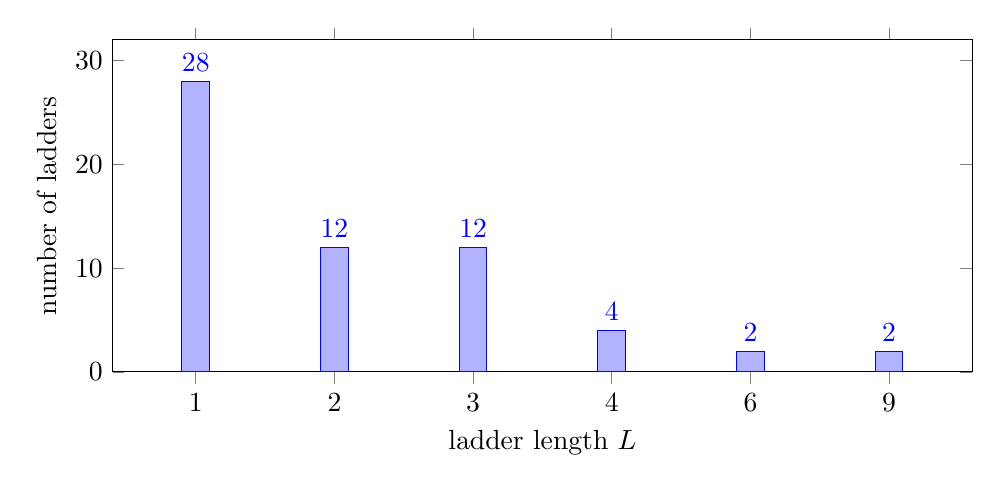
\begin{tikzpicture}
    \begin{axis}[
      ybar, bar width=10pt,
      width=12.5cm, height=5.8cm,
      ymin=0, ymax=32,
      symbolic x coords={1,2,3,4,6,9},
      xtick=data,
      xlabel={ladder length $L$},
      ylabel={number of ladders},
      nodes near coords,
      enlarge x limits=0.12,
    ]
    \addplot coordinates {(1,28) (2,12) (3,12) (4,4) (6,2) (9,2)};
    \end{axis}
  \end{tikzpicture}
  \caption{Ladder-length census from the R259 hole-twin hunt: $202$
    hole-twin pairs ($46/46$ ledger positive control), $134$ single-gap,
    $60$ ladders in total. The two $L=9$ ladders (\#49, \#59) are the
    catalog maxima (supplied datum, R259 dossier).}
  \label{fig:ladderbars}
\end{figure}

\begin{theorem}[Two-sided ladder ceiling; PROVED]
  \label{thm:ladder6}
  Let a hole-twin ladder $(X_t,Y_t)$, $t=0,\dots,L-1$, satisfy the
  one-sided hypotheses on each side: $t_0\le t_1$,
  $g_{\mathrm{prev}},g,g_{\mathrm{next}}\in G$,
  $g_{\mathrm{prev}}<g<g_{\mathrm{next}}$, and
  $\bigl([1-t_1,184-t_0]\cap G\bigr)=\{g\}$. Then
  \begin{equation}
    \label{eq:ladder6}
    L-1=t_1-t_0\le
    \min\bigl(g^a_{\mathrm{next}}-g^a_{\mathrm{prev}},
              g^b_{\mathrm{next}}-g^b_{\mathrm{prev}}\bigr)-185.
  \end{equation}
\end{theorem}

The one-sided core (\texttt{one\_sided\_ceiling}, [PROVED], axioms
\texttt{[propext, Quot.sound]}) is pure interval arithmetic: since
$g_{\mathrm{prev}}<g$ lies outside $[1-t_1,184-t_0]$ we have
$g_{\mathrm{prev}}\le-t_1$, and since $g<g_{\mathrm{next}}$ lies outside
we have $g_{\mathrm{next}}\ge185-t_0$; hence
$g_{\mathrm{next}}-g_{\mathrm{prev}}\ge185+(t_1-t_0)$, i.e.\
$t_1-t_0\le(g_{\mathrm{next}}-g_{\mathrm{prev}})-185$. Theorem~6
(\texttt{theorem6}) applies this to both sides and takes the minimum.
Rule-9 review SURVIVES, $12/12$ checks. Ladder~47 (R259) shows the bound
is sharp on one side: $L-1=5=190-185$ on the E10 march ($g_{\mathrm{next}}
-g_{\mathrm{prev}}=190$, supplied datum).

\begin{theorem}[Catalog ceiling; PROVED]
  \label{thm:catalog}
  Under Assumption~\ref{asm:ledger}, every hole-twin ladder over the
  $124$-oriented-base catalog satisfies
  \begin{equation}
    \label{eq:catalog}
    L\le9.
  \end{equation}
\end{theorem}

This is \texttt{catalog\_ceiling} (R263-a, [PROVED], axioms
\texttt{[propext, Quot.sound]}): with $L-1\le\min(\mathrm{iso}_A,
\mathrm{iso}_B)-185$ (Theorem~\ref{thm:ladder6}), $\min(\mathrm{iso}_A,
\mathrm{iso}_B)\le194$ [COMPUTED], the binding clause
$(\min=194\to L\le\mathrm{overlap})$ with $\mathrm{overlap}\le9$
[COMPUTED], we get $L-1\le9$ from the ceiling and, when the ceiling is
loose ($\min=194$), $L\le9$ from the overlap cap; otherwise
$\min\le193$ gives $L-1\le8$. The bound is attained: ladder~49
($L=9$, holes $19$--$27$, R47\#15 raw $t=-4..4$ gap~$23$ iso~$196$
$\times$ R47\#21 raw $t=-5..3$ gap~$24$ iso~$194$, $\delta=-1$;
[COMPUTED] datum, not formalized). Ladder~59 is the $\varphi$-dual
($L=9$, holes $158$--$166$). The ledger's distinct-base maximum
$194$ occurs only for R47\#15~$\times$~R47\#21 (raw$\times$raw and
$\varphi\times\varphi$); $8$ $L{=}10$-permitting rows exist in the raw
ledger ($6$ self $+$ $2$ binding), all vacuous on distinct bases
(supplied datum, R263 dossier).

%======================================================================
\section{Discussion}
%======================================================================

\paragraph{Significance.} The R245 identity generalizes the R223
sub-family theorem from the $f=1$ regime to arbitrary parameters:
where R223 gave expansions along a single parametric line,~\eqref{eq:general}
covers $1{,}239$ residue hits across eight new-regime shapes with $f>1$
(Table~\ref{tab:r245shapes}), each an explicit infinite family of
Erd\H{o}s--Straus expansions of the form~\eqref{eq:es}. The admission
criterion~\eqref{eq:AdmCond} turns a divisibility question into a
per-prime valuation check, and $A_0$-constancy collapses the
multi-$m$ moduli to a single shape-level $M(m)$ --- the mechanism behind
the same-modulus parent-set dichotomy. The ladder ceiling shows the
march-graph ladder machinery is self-limiting on the catalog:
$L\le9$ is both a theorem (Theorem~\ref{thm:catalog}) and an observed
fact (ladders~\#49, \#59).

\paragraph{The refutation record.} We keep it visible because the
repair is the point. R256's dichotomy review was MIXED (the arithmetic
and CRT arguments survived; the submitted proof was conditional on its
computed inputs, and the general ``$q\nmid m$'' premise failed on an
explicit admitted example). R261's $A_0$-constancy survived, but its
appended unconditional $\iff$ corollary was refuted as stated
(Proposition~\ref{prop:uncond-false}): three admitted values with empty
parent sets are both identical and disjoint. The surviving content is
the conditional, same-modulus form (Theorem~\ref{thm:split}), whose
determination premise remains Assumption~\ref{asm:determ}. This is the
honest boundary of the claim: no more is machine-checked.

\paragraph{Limitations.} (i) The [PROVED*] theorems are machine-checked
with zero sorrys and review-cleared, but their explicit full-library
label move is pending; they are presented as staged verification,
never as fully proved. (ii) The ladder ceiling's force is
catalog-relative: Theorem~\ref{thm:ladder6} is necessary but the
$L\le9$ bound depends on the ledger values of Assumption~\ref{asm:ledger};
$L\ge10$ stays [OPEN] and needs a new $\ge194$-isolation base. (iii)
The $82$ admitted-but-unobserved pairs ($49$ lemma-blocked with $0$
parents reaching, $33$ data-only vacuous) are all reclassified by R256
as visibility-blocked, but the \emph{existence} of parents in the
lemma-blocked cases is not established. (iv) The R245 setup's own
divisibility-collapse provenance (R72 TFAE, R209 parent residues) is
cited from program rounds, not re-derived; a reader meets the parameters
as given.

%======================================================================
\section{Conclusion}
%======================================================================

We have exhibited the generalized sub-family identity
(Theorem~\ref{thm:general}, [PROVED]), the valuation-form admission
criterion (Theorem~\ref{thm:admit}, [PROVED*]), the $A_0$-constancy
phenomenon with its excess-prime pinning (Theorem~\ref{thm:a0},
[PROVED*]), the conditional split/layered parent-set dichotomy
(Theorem~\ref{thm:split}, [PROVED*]) with the unconditional form's
refutation kept on the record (Proposition~\ref{prop:uncond-false}),
and the ladder ceilings $L-1\le\min(\mathrm{iso}_A,\mathrm{iso}_B)-185$
and $L\le9$ (Theorems~\ref{thm:ladder6} and~\ref{thm:catalog},
[PROVED]). The machine-checked results pass the bakkie build gate at
exit~$0$ with zero sorrys and standard-only axioms; the staged items
are labeled as such. The natural next steps are the full-library label
move for the [PROVED*] suite, a direct proof of the parent-set
determination premise (Assumption~\ref{asm:determ}), and the search for
a $\ge194$-isolation base that would test whether $L\ge10$ is
attainable.

%======================================================================
\section{References}
%======================================================================

\begin{thebibliography}{9}

\bibitem{ES48}
P.~Erd\H{o}s and E.~G.~Straus,
\emph{On the conjecture $4/n=1/x+1/y+1/z$},
unpublished manuscript, 1948.
(Cited as the classical conjecture of~\eqref{eq:es}; the program's
classical-literature reference set is cited as given.)

\bibitem{Mor69}
L.~J.~Mordell,
\emph{Diophantine equations},
Academic Press, 1969.
(Cited as given among the program's classical references.)

\bibitem{ET16}
C.~Elsholtz and T.~Tao,
counting results for the Erd\H{o}s--Straus equation,
cited as given in the program's classical-literature set.

\bibitem{Div26}
Divisor-parametrization reference, arXiv:2606.10922
(cited as given in the program's external prior-art list).

\bibitem{Dya25}
Dyachenko, arXiv:2511.07465
(cited as given in the program's external prior-art list).

\bibitem{D245}
D.~Blair,
\emph{Unsolved Math --- Round 245: generalized sub-family theorem},
program dossier, 2026-10-09.
(Supplied datum: identity setup, relation chain, eight new-regime
shapes, $1{,}239$ hits.)

\bibitem{D253}
D.~Blair,
\emph{Unsolved Math --- Round 253: admission criterion},
program dossier, 2026-10-10.
(Supplied datum: valuation criterion, $\times29$ cluster,
$154/154$ agreement.)

\bibitem{D256}
D.~Blair,
\emph{Unsolved Math --- Round 256: split/layered dichotomy},
program dossier, 2026-10-10.
(Supplied datum: parent-set machinery, census, MIXED review.)

\bibitem{D261}
D.~Blair,
\emph{Unsolved Math --- Round 261: $A_0$-constancy},
program dossier, 2026-10-10.
(Supplied datum: pinning mechanism, $781{,}250$-shape census,
refutation of the unconditional corollary.)

\bibitem{D262}
D.~Blair,
\emph{Unsolved Math --- Round 262: ESSubfamilyExtended formalized},
program dossier, 2026-10-10.
(Supplied datum: local+bakkie exit~0, zero sorrys, axiom audit,
md5s, reviewer's literal-statement counterexample.)

\bibitem{D259}
D.~Blair,
\emph{Unsolved Math --- Round 259: two-sided ladder ceiling},
program dossier, 2026-10-10.
(Supplied datum: ladder census, $60$ ladders, ladders~\#49/\#59/\#47.)

\bibitem{D263}
D.~Blair,
\emph{Unsolved Math --- Round 263: catalog ceiling ledger},
program dossier, 2026-10-10.
(Supplied datum: ceiling ledger, distinct-base maximum $194$,
overlap $\le9$, R263-a formalization.)

\bibitem{D310}
D.~Blair,
\emph{Unsolved Math --- Round 310: full-library build gate},
program dossier, 2026-10-11.
(Supplied datum: bakkie \texttt{lake build} ``Build completed
successfully (17936 jobs)'', exit~0, $0$ errors, $0$ sorrys;
[Q-12] label move.)

\end{thebibliography}

\end{document}

% --- WEAKNESSES (substantive) ---
% 1. The branch-1 identity is machine-checked, but the setup's provenance
%    (R72 TFAE, R209 parent residues) is cited from program rounds, not
%    re-derived: a reader meets q/e/f/u/D0 as given, not as motivated.
% 2. The parent-set determination premise (Assumption 1) is unproved and
%    its R256 review was MIXED; the conditional dichotomy floats on a
%    scaffold whose own foundations are not fully articulated here.
% 3. The L<=9 catalog ceiling depends on [COMPUTED] ledger values; the
%    paper risks being read as proving L<=9 about ladders per se, when it
%    is a theorem about this catalog's isolation data.
%
% --- TYPOGRAPHY ISSUES NOTICED ---
% 1. Inconsistent spacing around "mod" in residue-class displays
%    (s\equiv1041 (mod 1160) vs \pmod in equations) — should be uniform.
% 2. Mixed use of \texttt and math-roman for identifiers (M(m), A_excess,
%    AdmCond): the paper should settle on one convention for defined terms.
% 3. Several table cells mix math and text modes for multi-symbol entries
%    ("3, 39 / 3" with bare commas); thin spaces or a two-line cell would
%    typeset more cleanly.
